\documentclass[12pt,letterpaper]{article}
\usepackage{graphicx,textcomp}
\usepackage{natbib}
\usepackage{setspace}
\usepackage{fullpage}
\usepackage{color}
\usepackage[reqno]{amsmath}
\usepackage{amsthm}
\usepackage{fancyvrb}
\usepackage{amssymb,enumerate}
\usepackage[all]{xy}
\usepackage{endnotes}
\usepackage{adjustbox}
\usepackage{lscape}
\newtheorem{com}{Comment}
\usepackage{float}
\usepackage{hyperref}
\newtheorem{lem} {Lemma}
\newtheorem{prop}{Proposition}
\newtheorem{thm}{Theorem}
\newtheorem{defn}{Definition}
\newtheorem{cor}{Corollary}
\usepackage{enumitem}

\newtheorem{obs}{Observation}
\usepackage[compact]{titlesec}
\usepackage{dcolumn}
\usepackage{tikz}
\usetikzlibrary{arrows}
\usepackage{multirow}
\usepackage{xcolor}
\newcolumntype{.}{D{.}{.}{-1}}
\newcolumntype{d}[1]{D{.}{.}{#1}}
\definecolor{light-gray}{gray}{0.65}
\usepackage{url}
\usepackage{listings}
\usepackage{color}

\definecolor{codegreen}{rgb}{0,0.6,0}
\definecolor{codegray}{rgb}{0.5,0.5,0.5}
\definecolor{codepurple}{rgb}{0.58,0,0.82}
\definecolor{backcolour}{rgb}{0.95,0.95,0.92}

\lstdefinestyle{mystyle}{
	backgroundcolor=\color{backcolour},   
	commentstyle=\color{codegreen},
	keywordstyle=\color{magenta},
	numberstyle=\tiny\color{codegray},
	stringstyle=\color{codepurple},
	basicstyle=\footnotesize,
	breakatwhitespace=false,         
	breaklines=true,                 
	captionpos=b,                    
	keepspaces=true,                 
	numbers=left,                    
	numbersep=5pt,                  
	showspaces=false,                
	showstringspaces=false,
	showtabs=false,                  
	tabsize=2
}
\lstset{style=mystyle}
\newcommand{\Sref}[1]{Section~\ref{#1}}
\newtheorem{hyp}{Hypothesis}

\title{Answer Key: Problem Set 2}
\date{Jeffrey Ziegler}
\author{Applied Stats/Quant Methods 1}

\begin{document}
	\maketitle
	
	\section*{Instructions}
	\begin{itemize}
	\item \textit{Please show your work! You may lose points by simply writing in the answer. If the problem requires you to execute commands in \texttt{R}, please include the code you used to get your answers. Please also include the \texttt{.R} file that contains your code. If you are not sure if work needs to be shown for a particular problem, please ask.}
	\item \textit{Your homework should be submitted electronically on GitHub.}
	\item \textit{This problem set is due before 23:59 on Sunday October 15, 2023. No late assignments will be accepted.}
	\end{itemize}
	
	\vspace{.5cm}
	\section*{Question 1 (40 points): Political Science}
		\vspace{.25cm}
\textit{The following table was created using the data from a study run in a major Latin American city.\footnote{Fried, Brian J, Paul Lagunes, and Atheendar Venkataramani. 2010. "Corruption and Inequality at the Crossroad: A Multimethod Study of Bribery and Discrimination in Latin America". \textit{Latin American Research Review}. 45 (1): 76-97.} As part of the study, confederate made illegal left turns across traffic to draw the attention of the police officers.  Two of the confederates were upper class drivers and two were lower class drivers.  The researchers were interested in whether officers were more or less likely to solicit a bribe from drivers depending on their class (officers use phrases like, ``We can solve this the easy way'' to draw a bribe).  The table below shows the resulting data.}

\begin{table}[h!]
	\centering
	\begin{adjustbox}{max width=.75\textwidth}
		\begin{tabular}{l | c c c }
			& Not Stopped & Bribe requested & Stopped/given warning \\
			\\[-1.8ex] 
			\hline \\[-1.8ex]
			Upper class & 14 & 6 & 7 \\
			Lower class & 7 & 7 & 1 \\
			\hline
		\end{tabular}
	\end{adjustbox}
\end{table}

\begin{enumerate}
	
	\newpage
	\item [(a)]
	\textit{Calculate the $\chi^2$ test statistic by hand (even better if you can do "by hand" in \texttt{R}).}\\
	
	
	$$\text{Expected} =\frac{\sum_{\text{Row}}*\sum_{\text{Column}}}{\sum_{\text{N}}}$$
	$$\chi^2 = \sum_N \frac{\text{Observed}_i - \text{Expected}_i}{\text{Expected}_i}$$
	
	Let's first try by ourselves:		
	
	\lstinputlisting[language=R, firstline=40, lastline=77]{PS2_answerKey.R}  
	\footnotesize
	\begin{verbatim}
$statistic
[1] 3.791168

$df
[1] 2

$p.value
[1] 0.1502306

$observed
            Not_Stopped Bribe_Requested Stopped_Given_Warning
Upper_Class          14               6                     7
Lower_Class           7               7                     1

$expected
            Not_Stopped Bribe_Requested Stopped_Given_Warning
Upper_Class        13.5        8.357143              5.142857
Lower_Class         7.5        4.642857              2.857143

$adj_res
            Not_Stopped Bribe_Requested Stopped_Given_Warning
Upper_Class   0.3220306      -1.5164259             1.6491029
Lower_Class  -0.2740361       1.9295276            -1.5230259

$std_res
            Not_Stopped Bribe_Requested Stopped_Given_Warning
Upper_Class   0.3220306      -1.6419565             1.5230259
Lower_Class  -0.3220306       1.6419565            -1.5230259
	\end{verbatim}
	\normalsize
	Now we can check to make sure:
	
	\lstinputlisting[language=R, firstline=79, lastline=80]{PS2_answerKey.R}  
	\footnotesize
	\begin{verbatim}
	Pearson's Chi-squared test
	
	data:trafficViolations
	X-squared=3.7912, df=2, p-value=0.1502
	\end{verbatim}
	\normalsize
	\item [(b)]
	\textit{Now calculate the p-value (in \texttt{R}).\footnote{Remember frequency should be $>$ 5 for all cells, but let's calculate the p-value here anyway.}  What do you conclude if $\alpha = .1$?}\\
	
	\texttt{pchisq(3.79, df = (2-1)*(3-1), lower.tail = FALSE)} = 0.1502306\\

	P-value checks out to our "hand" calculation and the built in function. Cannot reject the null that the two variables of interest are independent.\\
	
			\vspace{.25cm}
	\item [(c)] \textit{Calculate the standardized residuals for each cell and put them in the table below.}\\
	
			\vspace{.15cm}
	We can do this by hand (see above function), or the standardized residuals are stored in the \texttt{chisq.test} object. We're reporting the standardized residuals, \texttt{(observed - expected) / sqrt(V)}, where $V$ is the residual cell variance (Agresti, 2007, section 2.4.5 for the case where $x$ is a matrix, $n * p * (1 - p)$ otherwise).\\

	\lstinputlisting[language=R, firstline=82, lastline=83]{PS2_answerKey.R}  
	
	
	\vspace{.25cm}
	\begin{table}[h!]
		\centering
		\begin{adjustbox}{max width=.75\textwidth}
			\begin{tabular}{l | c c c }
				& Not Stopped & Bribe requested & Stopped/given warning \\
				\\[-1.8ex] 
				\hline \\[-1.8ex]
				Upper class  & 0.322 & -1.642 & 1.523 \\
				\\
				Lower class & -0.322 & 1.642  & -1.523  \\
				
			\end{tabular}
		\end{adjustbox}
	\end{table}
	
		\vspace{.5cm}
	\item [(d)] \textit{How might the standardized residuals help you interpret the results?}  \\
	
			\vspace{.15cm}
	From the frequency table, it is already clear that there is no obvious pattern for a relationship between rows and columns. Further, the standardized residuals turn out to be quite small, which only supports us to be more confident about the lack of the dependency relationship. None of the standardized residuals indicate any of the cells are more or less than we would expect if the two variables were independent. Nevertheless, they do not tell us much, we need the chi-squared test to make conclusions in either case, i.e. whether variables are dependent or not.
	
\end{enumerate}

\newpage

\section*{Question 2 (20 points): Economics}
\textit{Chattopadhyay and Duflo were interested in studying the causal effect of having female politicians on policy outcomes.\footnote{Raghabendra Chattopadhyay and Esther Duflo. (2004). ``Women as Policy Makers: Evidence from a Randomized Policy Experiment in India. Econometrica, Vol. 72, No. 5, pp. 1409-1443.} Do women promote different policies than men? Answering this question with observational data is pretty difficult due to potential confounding problems (e.g. the districts that choose female politicians are likely to systematically differ in other aspects too). Hence, they exploit a randomized policy experiment in India, where since the mid-1990s, $\frac{1}{3}$ of village council heads have been {\bf{randomly}} reserved for women. A subset of the data from West Bengal can be found at the following link: \url{https://raw.githubusercontent.com/kosukeimai/qss/master/PREDICTION/women.csv}}\\

\noindent \textit{Each observation in the data set represents a village and there are two villages associated with one GP (i.e. a level of government is called "GP"). Figure~\ref{fig:women_desc} below shows the names and descriptions of the variables in the ``women.csv" dataset. The authors hypothesize that female politicians are more likely to support policies female voters want. Researchers found that more women complain about the quality of drinking water than men. You will be asked to estimate the effect of the reservation policy on the number of new or repaired drinking water facilities in the villages.}
\vspace{.5cm}
\begin{figure}[h!]
	\caption{\footnotesize{Names and description of variables from Chattopadhyay and Duflo (2004).}}
	\centering
	\label{fig:women_desc}
	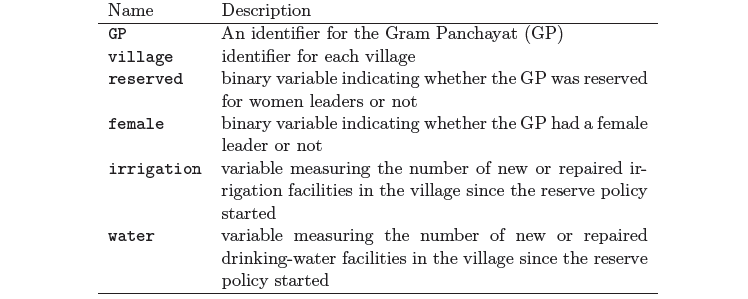
\includegraphics[width=1.1\textwidth]{../../../../graphics/women_desc.png}
\end{figure}		
\newpage
\begin{enumerate}
	\item [(a)] \textit{State a null and alternative (two-tailed) hypothesis. }
	
	Null: Having reserved seats for female politicians does not change the number drinking water facilities in the villages.\\
	
	Alternative: The reservation policy has an effect on policy outcomes.
	
	$$H_0: \beta = 0$$
	$$H_A: \beta \neq 0$$
%	\vspace{.05cm}
	
	\item [(b)] \textit{Run a bivariate regression to test this hypothesis in \texttt{R} (include your code!).}\\
	
					\vspace{.15cm}
	After we load our dataset into our working environment, we execute our regression model in which the number of new or repaired water facilities is explained by whether there are reserved seats for female leaders. We then investigate the estimated coefficients of the model using \texttt{summary()}.\\
	
					\vspace{.15cm}
	\lstinputlisting[language=R, firstline=89, lastline=94]{PS2_answerKey.R}  
	\begin{footnotesize}
		
		\begin{verbatim}
	Coefficients:
            Estimate Std. Error t value Pr(>|t|)    
(Intercept)   14.738      2.286   6.446 4.22e-10 ***
reserved       9.252      3.948   2.344   0.0197 *  
---
Signif. codes:  0 ‘***’ 0.001 ‘**’ 0.01 ‘*’ 0.05 ‘.’ 0.1 ‘ ’ 1
Residual standard error: 33.45 on 320 degrees of freedom
Multiple R-squared:  0.01688,	Adjusted R-squared:  0.0138 
F-statistic: 5.493 on 1 and 320 DF,  p-value: 0.0197
		\end{verbatim}
	\end{footnotesize}
	\item [(c)] \textit{Interpret the coefficient estimate for reservation policy.} 
	
				\vspace{.25cm}
	
	Having reserved seats for female politicians increase the number drinking water facilities in the villages, by 9.2 units. The estimated coefficient is statistically differentiable from zero at the $\alpha=0.05$ level because the p-value $<$ 0.05 ($\approx $0.02).
\end{enumerate}

\end{document}
